% https://tex.stackexchange.com/a/354987
\documentclass{beamer}

\usetheme{Madrid}      
\usecolortheme{beaver} 
\usepackage{tikz}
\usepackage{smartdiagram}

\begin{document}
\begin{frame}{Problématique} 
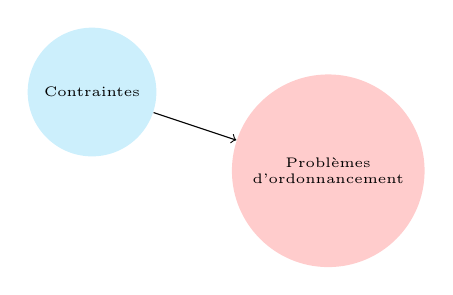
\begin{tikzpicture}[font=\tiny,fill,circle,minimum size=0.7cm,inner sep=5pt, align=center]
    \node[fill=red!20, text width=2cm] at (4,0) (A) {Problèmes d'ordonnancement};
    \node[fill=cyan!20] at (1,1) (B) {Contraintes};
    \draw [->] (B) -- (A);
\end{tikzpicture}
\end{frame}

\begin{frame}{test} 
\smartdiagramset{
    planet text width=2.5cm,
    satellite font=\scriptsize,
    bubble text opacity = 1,
    uniform connection color =true,
    connection color = bg
} 
\begin{center}
\scalebox{0.8}{
        \usebeamercolor{background canvas}
    \smartdiagram[constellation diagram]{
        Conditions de simulation,
        Type de tâches,
        Contraintes temporelles,
        Test de faisabilité du GEDF,
        Contraintes systèmes,
        Contraintes énergétiques
    }
}
\end{center}
\end{frame}


\end{document}
